\section{Consuntivo di periodo} \label{section:consuntivo}
Questa sezione riporta le spese effettivamente sostenute dal gruppo \groupName{}.
Vengono riportate le ore ed i costi impiegati in ciascun ruolo per svolgere le attività pianificate.
Viene inoltre presentato un bilancio in termini di costo, dato dalla differenza tra il consuntivo di periodo ed il preventivo, che potrà essere:
\begin{itemize}
  \item \textbf{Positivo:} Se la spesa effettiva è minore di quanto preventivato;
  \item \textbf{In pareggio:} Se la spesa effettiva è uguale a quanto preventivato;
  \item \textbf{Negativo:} Se la spesa effettiva è maggiore di quanto preventivato.
\end{itemize}
Il bilancio viene riportato tra parentesi a fianco dei valori rilevati dal consuntivo di periodo.\\
Se il valore tra parentesi non è presente indica che l'aspettativa del preventivo è stata rispettata.

%%%%%%%%%%%%%%%%%%%%%%%%%%%%%%%%%%%%%%%%%%%%%%%%%%%%%%%%%%%%%%

\subsection{Analisi preliminare} \label{subsection:consuntivo_analisi}
\subsubsection{Variazione della pianificazione} \label{subsubsection:variazione_pianificazione_analisi}
\begin{table}[H]
  \centering
  \renewcommand{\arraystretch}{1.8}
  \rowcolors{2}{green!100!black!40}{green!100!black!30}
  \begin{tabular}{c|c|c|c|c|c|c|c}
    \rowcolor[HTML]{125E28}
    \multicolumn{1}{c}{\color[HTML]{FFFFFF}\textbf{Nominativo}}
                         & \multicolumn{1}{c}{\color[HTML]{FFFFFF}\textbf{ Re }}
                         & \multicolumn{1}{c}{\color[HTML]{FFFFFF}\textbf{ Am}}
                         & \multicolumn{1}{c}{\color[HTML]{FFFFFF}\textbf{ An }}
                         & \multicolumn{1}{c}{\color[HTML]{FFFFFF}\textbf{ Pt }}
                         & \multicolumn{1}{c}{\color[HTML]{FFFFFF}\textbf{ Pr }}
                         & \multicolumn{1}{c}{\color[HTML]{FFFFFF}\textbf{ Ve }}
                         & \multicolumn{1}{c}{\color[HTML]{FFFFFF}\textbf{ Ore totali }}                                                                                                        \\
    \hline
    Bugno Francesco      & 11 (+2)                                                       & -                & 9                & -          & -          & 11 (-2)          & 31                \\
    Busacca Luca         & -                                                             & 17               & 5                & -          & -          & 9  (-1)          & 31 (-1)           \\
    Carturan Luca        & 12 (+1)                                                       & 5 (+1)           & 5                & -          & -          & 9  (-2)          & 31                \\
    Filosofo Michele     & -                                                             & 5 (+2)           & 15 (-2)          & -          & -          & 11               & 31                \\
    Furlan Dario         & -                                                             & -                & 19 (-1)          & -          & -          & 12               & 31 (-1)           \\
    Mattarello Francesco & -                                                             & 15               & 6                & -          & -          & 10 (-1)          & 31 (-1)           \\
    Midena Matteo        & -                                                             & -                & 23 (-1)          & -          & -          & 9                & 32 (-1)           \\
    \textbf{Ore totali}  & \textbf{23 (+3)}                                              & \textbf{43 (+3)} & \textbf{82 (-4)} & \textbf{-} & \textbf{-} & \textbf{71 (-6)} & \textbf{218 (-4)}
  \end{tabular}
  \caption{Variazione delle ore nel periodo di Analisi preliminare}
\end{table}

\subsubsection{Variazione dei costi} \label{subsubsection:variazione_costi_analisi}
\begin{table}[H]
  \centering
  \renewcommand{\arraystretch}{1.8}
  \rowcolors{2}{green!100!black!40}{green!100!black!30}
  \begin{tabular}{c|c|c}
    \rowcolor[HTML]{125E28}
    \multicolumn{1}{c}{\color[HTML]{FFFFFF}\textbf{Ruolo}}
                               & \multicolumn{1}{c}{\color[HTML]{FFFFFF}\textbf{Ore}}
                               & \multicolumn{1}{c}{\color[HTML]{FFFFFF}\textbf{Costo (€)}}                     \\
    \hline
    Responsabile               & 23 (+3)                                                    & 690,00 (+90,00)   \\
    Amministratore             & 42 (+3)                                                    & 840,00 (+60,00)   \\
    Analista                   & 82 (-4)                                                    & 2050,00 (-100,00) \\
    Progettista                & -                                                          & -                 \\
    Programmatore              & -                                                          & -                 \\
    Verificatore               & 71 (-6)                                                    & 1065,00 (-90,00)  \\
    \textbf{Totale Consuntivo} & \textbf{214}                                               & \textbf{4605,00}  \\
    \textbf{Totale Preventivo} & \textbf{218}                                               & \textbf{4645,00}  \\
    \textbf{Bilancio}          & \textbf{-4}                                                & \textbf{-40,00}   \\
  \end{tabular}
  \caption{Analisi preliminare - Consuntivo di periodo}
\end{table}


\subsubsection{Ragione degli scostamenti} \label{subsubsection:ragione_scostamenti_analisi}
\begin{itemize}
  \item \textbf{Responsabile (+3 ore):} Inizialmente, a causa dell'inesperienza, tale figura ha riscontrato problemi nella suddivisione del carico del lavoro, richiedendo un'analisi più minuziosa;
  \item \textbf{Amministratore (+3 ore):} La stesura delle \docNameNdP{} ha richiesto più tempo del previsto data l'elevata dipendenza con gli altri documenti;
  \item \textbf{Analista (-4 ore):} Grazie alle conoscenze pregresse di alcuni membri del gruppo si è riusciti ad ottimizzare i tempi previsti per l'\docNameAdR{};
  \item \textbf{Verificatore (-6 ore):} Durante questo periodo, avendo solamente documentazione da verificare, il controllo è risultato più rapido del previsto.
\end{itemize}

\subsubsection{Considerazioni rispetto al preventivo} \label{subsubsection:considerazioni_finali_analisi}
Il bilancio risulta essere positivo rispetto al preventivo per questo periodo. Non si ritiene comunque necessaria alcuna ripianificazione del prossimo periodo in quanto la somma risparmiata non è abbastanza significativa.
Inoltre, avendo raggiunto tutti gli obiettivi precedentemente pianificati, l'avanzamento delle attività non ha subito alcun rallentamento.
\pagebreak
%%%%%%%%%%%%%%%%%%%%%%%%%%%%%%%%%%%%%%%%%%%%%%%%%%%%%%%%%%%%%%

\subsection{Progettazione Technology Baseline} \label{subsection:consuntivo_TB}
\subsubsection{Variazione della pianificazione} \label{subsubsection:variazione_pianificazione_TB}

\begin{table}[H]
  \centering
  \renewcommand{\arraystretch}{1.8}
  \rowcolors{2}{green!100!black!40}{green!100!black!30}
  \begin{tabular}{c|c|c|c|c|c|c|c}
    \rowcolor[HTML]{125E28}
    \multicolumn{1}{c}{\color[HTML]{FFFFFF}\textbf{ Nominativo }}
                         & \multicolumn{1}{c}{\color[HTML]{FFFFFF}\textbf{ Re }}
                         & \multicolumn{1}{c}{\color[HTML]{FFFFFF}\textbf{ Am}}
                         & \multicolumn{1}{c}{\color[HTML]{FFFFFF}\textbf{ An }}
                         & \multicolumn{1}{c}{\color[HTML]{FFFFFF}\textbf{ Pt }}
                         & \multicolumn{1}{c}{\color[HTML]{FFFFFF}\textbf{ Pr }}
                         & \multicolumn{1}{c}{\color[HTML]{FFFFFF}\textbf{ Ve }}
                         & \multicolumn{1}{c}{\color[HTML]{FFFFFF}\textbf{ Ore totali }}                                                                                                             \\
    \hline
    Bugno Francesco      & -                                                             & 2               & 3                & 3 (-1)           & -          & 3 (-1)           & 11 (-2)           \\
    Busacca Luca         & -                                                             & -               & -                & 6 (-1)           & -          & 4 (-1)           & 10 (-2)           \\
    Carturan Luca        & -                                                             & -               & 5 (-1)           & 6 (-1)           & -          & -                & 11 (-2)           \\
    Filosofo Michele     & -                                                             & 3               & -                & 4 (-1)           & -          & 4 (-1)           & 11 (-2)           \\
    Furlan Dario         & 7 (-2)                                                        & -               & -                & 5                & -          & -                & 12 (-2)           \\
    Mattarello Francesco & -                                                             & -               & 4                & 4 (-1)           & -          & 3 (-1)           & 11 (-2)           \\
    Midena Matteo        & -                                                             & 3 (-1)          & -                & 5 (-1)           & -          & 3                & 11 (-2)           \\
    \textbf{Ore totali}  & \textbf{7 (-2)}                                               & \textbf{8 (-1)} & \textbf{12 (-1)} & \textbf{33 (-6)} & \textbf{-} & \textbf{17 (-4)} & \textbf{77 (-14)}
  \end{tabular}
  \caption{Variazione delle ore nel periodo di Progettazione Technology Baseline}
\end{table}

\subsubsection{Variazione dei costi} \label{subsubsection:variazione_costi_TB}

\begin{table}[H]
  \centering
  \renewcommand{\arraystretch}{1.8}
  \rowcolors{2}{green!100!black!40}{green!100!black!30}
  \begin{tabular}{c|c|c}
    \rowcolor[HTML]{125E28}
    \multicolumn{1}{c}{\color[HTML]{FFFFFF}\textbf{Ruolo}} &
    \multicolumn{1}{c}{\color[HTML]{FFFFFF}\textbf{Ore}}   &
    \multicolumn{1}{c}{\color[HTML]{FFFFFF}\textbf{Costo (€)}}                               \\
    \hline
    Responsabile                                           & 7 (-2)       & 210,00 (-60,00)  \\
    Amministratore                                         & 8 (-1)       & 160,00 (-20,00)  \\
    Analista                                               & 12 (-1)      & 300,00 (-25,00)  \\
    Progettista                                            & 33 (-6)      & 825,00 (-150,00) \\
    Programmatore                                          & -            & -                \\
    Verificatore                                           & 17 (-4)      & 255,00 (-60,00)  \\
    \textbf{Totale Consuntivo}                             & \textbf{63}  & \textbf{1435,00} \\
    \textbf{Totale Preventivo}                             & \textbf{77}  & \textbf{1750,00} \\
    \textbf{Bilancio}                                      & \textbf{-14} & \textbf{-315,00} \\
  \end{tabular}
  \caption{Progettazione Technology Baseline - Consuntivo di periodo}
\end{table}


\subsubsection{Ragione degli scostamenti} \label{subsubsection:ragione_scostamenti_TB}
A causa dell'inizio della sessione d'esame si è deciso di apportare una variazione della pianificazione inizialmente preventivata per dare la possibilità ai singoli membri del gruppo di potersi dedicare allo studio individuale.
Di comune accordo si è pensato di ridurre per ciascun membro le ore totali da dedicare al progetto in modo equilibrato e sensato per non stravolgere il normale flusso di lavoro.

\subsubsection{Considerazioni rispetto al preventivo} \label{subsubsection:considerazioni_finali_TB}
Il bilancio risulta essere positivo rispetto al preventivo per questo periodo.
A causa del minor tempo che il gruppo è riuscito a dedicare al progetto in questo periodo si è ritenuto necessaria una ripianificazione del periodo successivo.
Non avendo raggiunto tutti gli obiettivi precedentemente pianificati il gruppo ha deciso di attribuire maggiore importanza al ruolo di \roleDesignerLow{} e \roleProgrammerLow{}, incrementandone le ore di lavoro, per riuscire a rispettare il più possibile la pianificazione iniziale e non sforare con le tempistiche.

\paragraph{Codifica Proof of Concept - Preventivo a finire} \label{paragraph:preventivo_finire_Poc}

\subparagraph{Prospetto orario} \label{subparagraph:prospetto_orario_PoC}
\begin{table}[H]
  \centering
  \renewcommand{\arraystretch}{1.8}
  \rowcolors{2}{green!100!black!40}{green!100!black!30}
  \begin{tabular}{c|c|c|c|c|c|c|c}
    \rowcolor[HTML]{125E28}
    \multicolumn{1}{c}{\color[HTML]{FFFFFF}\textbf{ Nominativo }}
                         & \multicolumn{1}{c}{\color[HTML]{FFFFFF}\textbf{ Re }}
                         & \multicolumn{1}{c}{\color[HTML]{FFFFFF}\textbf{ Am}}
                         & \multicolumn{1}{c}{\color[HTML]{FFFFFF}\textbf{ An }}
                         & \multicolumn{1}{c}{\color[HTML]{FFFFFF}\textbf{ Pt }}
                         & \multicolumn{1}{c}{\color[HTML]{FFFFFF}\textbf{ Pr }}
                         & \multicolumn{1}{c}{\color[HTML]{FFFFFF}\textbf{ Ve }}
                         & \multicolumn{1}{c}{\color[HTML]{FFFFFF}\textbf{ Ore totali }}                                                                                                          \\
    \hline
    Bugno Francesco      & -                                                             & -               & -          & 7 (+1)            & 4 (+2)           & 6           & 17 (+3)            \\
    Busacca Luca         & -                                                             & -               & 3          & 5 (+2)            & 7                & 4           & 19 (+2)            \\
    Carturan Luca        & -                                                             & -               & -          & 6 (+1)            & 8 (+2)           & 3           & 17 (+3)            \\
    Filosofo Michele     & -                                                             & -               & 4          & 4 (+2)            & 7                & 3           & 18 (+2)            \\
    Furlan Dario         & -                                                             & 2               & -          & 8 (+1)            & 8 (+1)           & -           & 18 (+2)            \\
    Mattarello Francesco & -                                                             & 3 (-1)          & -          & 6 (+1)            & 2 (+2)           & 7           & 18 (+2)            \\
    Midena Matteo        & 8 (-2)                                                        & -               & -          & 2 (+3)            & 8 (+1)           & -           & 18 (+2)            \\
    \textbf{Ore totali}  & \textbf{8 (-2)}                                               & \textbf{5 (-1)} & \textbf{7} & \textbf{38 (+11)} & \textbf{44 (+8)} & \textbf{23} & \textbf{125 (+16)}
  \end{tabular}
  \caption{Distribuzione delle ore nel periodo di Codifica Proof of Concept - Preventivo a finire}
\end{table}

I valori sono riassunti graficamente nel seguente grafico:
\begin{figure}[H]
  \centering
  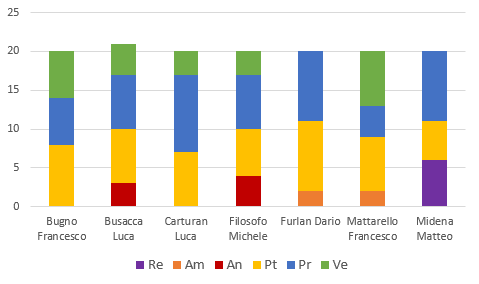
\includegraphics[scale=0.9]{immagini/ore_lavoro_preventivo_finire_PoC.png}
  \caption{Distribuzione ore di lavoro periodo di Codifica Proof of Concept - Preventivo a finire}
\end{figure}

\subparagraph{Prospetto economico} \label{subparagraph:prospetto_economico_PoC}

\begin{table}[H]
  \centering
  \renewcommand{\arraystretch}{1.8}
  \rowcolors{2}{green!100!black!40}{green!100!black!30}
  \begin{tabular}{c|c|c}
    \rowcolor[HTML]{125E28}
    \multicolumn{1}{c}{\color[HTML]{FFFFFF}\textbf{Ruolo}}
                    & \multicolumn{1}{c}{\color[HTML]{FFFFFF}\textbf{Ore}}
                    & \multicolumn{1}{c}{\color[HTML]{FFFFFF}\textbf{Costo (€)}}                              \\
    \hline
    Responsabile    & 8 (-2)                                                     & 240,00 (-60,00)            \\
    Amministratore  & 5 (-1)                                                     & 100,00 (-20,00)            \\
    Analista        & 7                                                          & 175,00                     \\
    Progettista     & 38 (+11)                                                   & 950,00 (+275,00)           \\
    Programmatore   & 44 (+8)                                                    & 660,00 (+120,00)           \\
    Verificatore    & 23                                                         & 345,00                     \\
    \textbf{Totale} & \textbf{141 (+16)}                                         & \textbf{2470,00 (+315,00)} \\
  \end{tabular}
  \caption{Prospetto delle ore e dei costi per ruolo nel periodo di Codifica Proof of Concept - Preventivo a finire}
\end{table}

\begin{figure}[H]
  \centering
  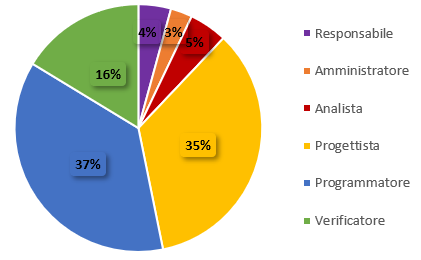
\includegraphics[scale=0.9]{immagini/ore_ruolo_preventivo_finire_PoC.png}
  \caption{Suddivisione delle ore di lavoro per ruolo sul totale per il periodo di Codifica Proof of Concept- Preventivo a finire}
\end{figure}


%%%%%%%%%%%%%%%%%%%%%%%%%%%%%%%%%%%%%%%%%%%%%%%%%%%%%%%%%%%%%%

\paragraph{Progettazione di dettaglio e codifica requisiti obbligatori - Preventivo a finire} \label{paragraph:preventivo_finire_reqObbligatori}
Per ora la pianificazione di questo periodo rimane invariata rispetto a quella iniziale.
Successivamente alla revisione \RTB{}, se necessario, verrà aggiornata la pianificazione riguardante questo periodo.
\paragraph{Progettazione di dettaglio e codifica requisiti opzionali - Preventivo a finire} \label{paragraph:preventivo_finire_reqOpzionali}
Per ora la pianificazione di questo periodo rimane invariata rispetto a quella iniziale.
Successivamente alla revisione \RTB{}, se necessario, verrà aggiornata la pianificazione riguardante questo periodo.
\paragraph{Validazione e collaudo - Preventivo a finire} \label{paragraph:preventivo_finire_Validazione}
Per ora la pianificazione di questo periodo rimane invariata rispetto a quella iniziale.
Successivamente alla revisione \RTB{}, se necessario, verrà aggiornata la pianificazione riguardante questo periodo.

\subsubsection{Conclusioni} \label{subsubsection:conclusioni}
Il totale delle ore rendicontate preventivate per il progetto diventa il seguente:

\begin{table}[H]
  \centering
  \renewcommand{\arraystretch}{1.8}
  \rowcolors{2}{green!100!black!40}{green!100!black!30}
  \begin{tabular}{c|c|c|c|c|c|c|c}
    \rowcolor[HTML]{125E28}
    \multicolumn{1}{c}{\color[HTML]{FFFFFF}\textbf{ Nominativo }}
                         & \multicolumn{1}{c}{\color[HTML]{FFFFFF}\textbf{ Re }}
                         & \multicolumn{1}{c}{\color[HTML]{FFFFFF}\textbf{ Am}}
                         & \multicolumn{1}{c}{\color[HTML]{FFFFFF}\textbf{ An }}
                         & \multicolumn{1}{c}{\color[HTML]{FFFFFF}\textbf{ Pt }}
                         & \multicolumn{1}{c}{\color[HTML]{FFFFFF}\textbf{ Pr }}
                         & \multicolumn{1}{c}{\color[HTML]{FFFFFF}\textbf{ Ve }}
                         & \multicolumn{1}{c}{\color[HTML]{FFFFFF}\textbf{ Ore totali }}                                                                                                                         \\
    \hline
    Bugno Francesco      & 11 (+2)                                                       & 5                & 12                & 20                & 23 (+2)           & 29 (-3)            & 100 (+1)          \\
    Busacca Luca         & 4                                                             & 17               & 10                & 20 (+1)           & 25                & 24 (-2)            & 100 (-1)          \\
    Carturan Luca        & 12 (+1)                                                       & 5 (+1)           & 10 (-1)           & 23                & 28 (+2)           & 22 (-2)            & 100 (+1)          \\
    Filosofo Michele     & 6                                                             & 8 (+2)           & 19 (-2)           & 24 (+1)           & 17                & 26 (-1)            & 100               \\
    Furlan Dario         & 7 (-2)                                                        & 10               & 19 (-1)           & 24 (+1)           & 15 (+1)           & 25                 & 100 (-1)          \\
    Mattarello Francesco & 7                                                             & 18 (-1)          & 12                & 23                & 16 (+2)           & 24 (-2)            & 100 (-1)          \\
    Midena Matteo        & 8 (-2)                                                        & 7 (-1)           & 23 (-1)           & 16 (+2)           & 26 (+1)           & 20                 & 100 (-1)          \\
    \textbf{Ore totali}  & \textbf{55 (-1)}                                              & \textbf{70 (+1)} & \textbf{105 (-5)} & \textbf{150 (+5)} & \textbf{150 (+8)} & \textbf{170 (-10)} & \textbf{700 (-2)}
  \end{tabular}
  \caption{Riepilogo della distribuzione oraria totale rendicontata - Preventivo a finire}
\end{table}

\begin{figure}[H]
  \centering
  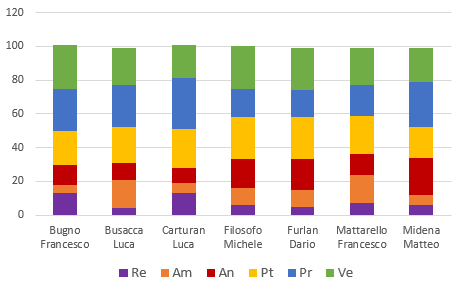
\includegraphics[scale=0.9]{immagini/ore_lavoro_preventivo_finire.png}
  \caption{Istogramma della distribuzione oraria totale rendicontata - Preventivo a finire}
\end{figure}


\begin{table}[H]
  \centering
  \renewcommand{\arraystretch}{1.8}
  \rowcolors{2}{green!100!black!40}{green!100!black!30}
  \begin{tabular}{c|c|c}
    \rowcolor[HTML]{125E28}
    \multicolumn{1}{c}{\color[HTML]{FFFFFF}\textbf{Ruolo}}
                    & \multicolumn{1}{c}{\color[HTML]{FFFFFF}\textbf{Ore}}
                    & \multicolumn{1}{c}{\color[HTML]{FFFFFF}\textbf{Costo (€)}}                              \\
    \hline
    Responsabile    & 55 (-1)                                                    & 1650,00 (-30,00)           \\
    Amministratore  & 70 (+1)                                                    & 1400,00 (+20,00)           \\
    Analista        & 105 (-5)                                                   & 2625,00 (-125,00)          \\
    Progettista     & 150 (+5)                                                   & 3750,00 (+125,00)          \\
    Programmatore   & 150 (+8)                                                   & 2250,00 (+120,00)          \\
    Verificatore    & 170 (-10)                                                  & 2550,00 (-150,00)          \\
    \textbf{Totale} & \textbf{700 (-2)}                                          & \textbf{14225,00 (-40,00)} \\
  \end{tabular}
  \caption{Prospetto delle ore e dei costi delle ore rendicontate - Preventivo a finire}
\end{table}

\begin{figure}[H]
  \centering
  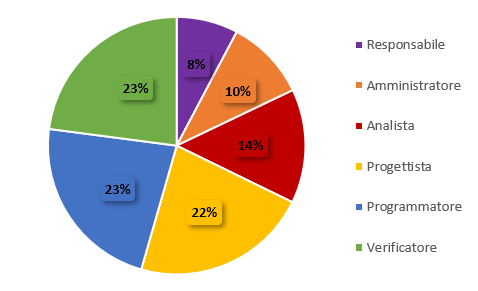
\includegraphics[scale=0.9]{immagini/ore_ruolo_preventivo_finire.png}
  \caption{Areogramma delle ore per ruolo rendicontate sul totale - Preventivo a finire}
\end{figure}

Il carico di ore a persona è leggermente diminuito e il preventivo a finire scende a 14185,00€.

\pagebreak
%%%%%%%%%%%%%%%%%%%%%%%%%%%%%%%%%%%%%%%%%%%%%%%%%%%%%%%%%%%%%%

\subsection{Codifica Proof of Concept} \label{subsection:consuntivo_PoC}
\subsubsection{Variazione della pianificazione} \label{subsubsection:variazione_pianificazione_PoC}

\begin{table}[H]
  \centering
  \renewcommand{\arraystretch}{1.8}
  \rowcolors{2}{green!100!black!40}{green!100!black!30}
  \begin{tabular}{c|c|c|c|c|c|c|c}
    \rowcolor[HTML]{125E28}
    \multicolumn{1}{c}{\color[HTML]{FFFFFF}\textbf{ Nominativo }}
                         & \multicolumn{1}{c}{\color[HTML]{FFFFFF}\textbf{ Re }}
                         & \multicolumn{1}{c}{\color[HTML]{FFFFFF}\textbf{ Am}}
                         & \multicolumn{1}{c}{\color[HTML]{FFFFFF}\textbf{ An }}
                         & \multicolumn{1}{c}{\color[HTML]{FFFFFF}\textbf{ Pt }}
                         & \multicolumn{1}{c}{\color[HTML]{FFFFFF}\textbf{ Pr }}
                         & \multicolumn{1}{c}{\color[HTML]{FFFFFF}\textbf{ Ve }}
                         & \multicolumn{1}{c}{\color[HTML]{FFFFFF}\textbf{ Ore totali }}                                                                                                             \\
    \hline
    Bugno Francesco      & -                                                             & -          & - (+2)          & 8 (-2)           & 6                & 6                & 20                \\
    Busacca Luca         & -                                                             & -          & 3 (+1)          & 7 (-1)           & 7 (-1)           & 4 (+1)           & 21                \\
    Carturan Luca        & -                                                             & -          & -               & 7                & 10 (-3)          & 3 (+3)           & 20                \\
    Filosofo Michele     & -                                                             & -          & 4               & 6                & 7 (-2)           & 3 (+2)           & 20                \\
    Furlan Dario         & -                                                             & 2          & -               & 9 (-1)           & 9 (+1)           & -                & 20                \\
    Mattarello Francesco & -                                                             & 2          & -               & 7                & 4                & 7                & 20                \\
    Midena Matteo        & 6                                                             & -          & -               & 5                & 9 (+1)           & -                & 20 (+1)           \\
    \textbf{Ore totali}  & \textbf{6}                                                    & \textbf{4} & \textbf{7 (+3)} & \textbf{49 (-4)} & \textbf{52 (-4)} & \textbf{23 (+6)} & \textbf{141 (+1)}
  \end{tabular}
  \caption{Variazione delle ore nel periodo di Codifica Proof of Concept}
\end{table}

\subsubsection{Variazione dei costi} \label{subsubsection:variazione_costi_Poc}

\begin{table}[H]
  \centering
  \renewcommand{\arraystretch}{1.8}
  \rowcolors{2}{green!100!black!40}{green!100!black!30}
  \begin{tabular}{c|c|c}
    \rowcolor[HTML]{125E28}
    \multicolumn{1}{c}{\color[HTML]{FFFFFF}\textbf{Ruolo}} &
    \multicolumn{1}{c}{\color[HTML]{FFFFFF}\textbf{Ore}}   &
    \multicolumn{1}{c}{\color[HTML]{FFFFFF}\textbf{Costo (€)}}                                \\
    \hline
    Responsabile                                           & 6            & 180,00            \\
    Amministratore                                         & 4            & 80,00             \\
    Analista                                               & 7 (+3)       & 175,00 (+75,00)   \\
    Progettista                                            & 49 (-4)      & 1225,00 (-100,00) \\
    Programmatore                                          & 52 (-4)      & 780,00 (-60,00)   \\
    Verificatore                                           & 23 (+6)      & 345,00 (+90,00)   \\
    \textbf{Totale Consuntivo}                             & \textbf{142} & \textbf{2790,00}  \\
    \textbf{Totale Preventivo}                             & \textbf{141} & \textbf{2785,00}  \\
    \textbf{Bilancio}                                      & \textbf{+1}  & \textbf{+5,00}    \\
  \end{tabular}
  \caption{Codifica Proof of Concept - Consuntivo di periodo}
\end{table}

\pagebreak
\subsubsection{Ragione degli scostamenti} \label{subsubsection:ragione_scostamenti_PoC}
Inizialmente il gruppo si è concentrato nel suddividere in modo opportuno gli incrementi precedentemente individuati.
Queste accortezze hanno portato inevitabilmente un aumento delle ore al ruolo di \roleAnalystLow{}.
Infine, grazie alla conoscenza pregressa dei linguaggi di programmazione utilizzati da parte di alcuni membri del gruppo, la codifica del PoC\glo{} ha richiesto meno tempo del previsto, permettendo di ripartire le ore degli altri componenti alla verifica della documentazione.
Per questi motivi c'è stata la rispettiva diminuzione di ore al ruolo di \roleDesignerLow{} e \roleProgrammerLow{}, con conseguente incremento al ruolo di \roleVerifierLow{}.

\subsubsection{Considerazioni rispetto al preventivo} \label{subsubsection:considerazioni_finali_PoC}
Il bilancio risulta essere negativo di 5,00€ rispetto al preventivo per questo periodo.
Non si ritiene comunque necessaria alcuna ripianificazione in quanto la somma sforata viene ampiamente ricoperta dal risparmio di 40,00€ del precedente periodo.
Inoltre, avendo raggiunto tutti gli obiettivi pianificati, l'avanzamento delle attività non ha subito alcun rallentamento.

\subsection{Esito colloquio Technology Baseline} \label{subsubsection:esito_TB}
A causa del semaforo rosso ricevuto al primo colloquio con il \commitNameS{}, il gruppo ha dovuto effettuare delle modifiche migliorative riguardanti l'\docNameAdR{} \textit{v1.0.0}.\\
Ciò ha comportato un incremento delle ore lavorative per tutti i componenti del gruppo, il quale non verrà preso in considerazione nei calcoli delle ore da rendicontare in quanto dovuto a errori commessi dal gruppo \groupName{}.
\pagebreak
%%%%%%%%%%%%%%%%%%%%%%%%%%%%%%%%%%%%%%%%%%%%%%%%%%%%%%%%%%%%%%

\subsection{Sprint 1 - Progettazione di dettaglio e codifica dei requisiti} \label{subsection:consuntivo_sprint1}
\subsubsection{Variazione della pianificazione} \label{subsubsection:variazione_pianificazione_sprint1}

\begin{table}[H]
  \centering
  \renewcommand{\arraystretch}{1.8}
  \rowcolors{2}{green!100!black!40}{green!100!black!30}
  \begin{tabular}{c|c|c|c|c|c|c|c}
    \rowcolor[HTML]{125E28}
    \multicolumn{1}{c}{\color[HTML]{FFFFFF}\textbf{ Nominativo }}
                         & \multicolumn{1}{c}{\color[HTML]{FFFFFF}\textbf{ Re }}
                         & \multicolumn{1}{c}{\color[HTML]{FFFFFF}\textbf{ Am}}
                         & \multicolumn{1}{c}{\color[HTML]{FFFFFF}\textbf{ An }}
                         & \multicolumn{1}{c}{\color[HTML]{FFFFFF}\textbf{ Pt }}
                         & \multicolumn{1}{c}{\color[HTML]{FFFFFF}\textbf{ Pr }}
                         & \multicolumn{1}{c}{\color[HTML]{FFFFFF}\textbf{ Ve }}
                         & \multicolumn{1}{c}{\color[HTML]{FFFFFF}\textbf{ Ore totali }}                                                                                                            \\
    \hline
    Bugno Francesco      & -                                                             & -          & -               & 3                & 4                & 2 (-1)           & 9 (-1)           \\
    Busacca Luca         & -                                                             & -          & 2 (-1)          & -                & 4                & 3                & 9 (-1)           \\
    Carturan Luca        & -                                                             & -          & 0 (-1)          & 3                & 3 (-1)           & 3                & 9 (-2)           \\
    Filosofo Michele     & 4                                                             & -          & -               & 3                & -                & 2 (-1)           & 9 (-1)           \\
    Furlan Dario         & -                                                             & 3          & -               & 3 (-1)           & -                & 3                & 9 (-1)           \\
    Mattarello Francesco & -                                                             & -          & 0 (-1)          & 4                & 5                & -                & 9 (-1)           \\
    Midena Matteo        & -                                                             & -          & 0 (-1)          & 4                & 5 (-1)           & -                & 9 (-2)           \\
    \textbf{Ore totali}  & \textbf{4}                                                    & \textbf{3} & \textbf{2 (-4)} & \textbf{20 (-1)} & \textbf{21 (-2)} & \textbf{13 (-2)} & \textbf{63 (-9)}
  \end{tabular}
  \caption{Variazione delle ore nel primo Sprint}
\end{table}

\subsubsection{Variazione dei costi} \label{subsubsection:variazione_costi_sprint1}

\begin{table}[H]
  \centering
  \renewcommand{\arraystretch}{1.8}
  \rowcolors{2}{green!100!black!40}{green!100!black!30}
  \begin{tabular}{c|c|c}
    \rowcolor[HTML]{125E28}
    \multicolumn{1}{c}{\color[HTML]{FFFFFF}\textbf{Ruolo}} &
    \multicolumn{1}{c}{\color[HTML]{FFFFFF}\textbf{Ore}}   &
    \multicolumn{1}{c}{\color[HTML]{FFFFFF}\textbf{Costo (€)}}                              \\
    \hline
    Responsabile                                           & 4           & 120,00           \\
    Amministratore                                         & 3           & 60,00            \\
    Analista                                               & 2 (-4)      & 50,00 (-100,00)  \\
    Progettista                                            & 20 (-1)     & 500,00 (-25,00)  \\
    Programmatore                                          & 21 (-2)     & 315,00 (-30,00)  \\
    Verificatore                                           & 13 (-2)     & 195,00 (-30,00)  \\
    \textbf{Totale Consuntivo}                             & \textbf{63} & \textbf{1240,00} \\
    \textbf{Totale Preventivo}                             & \textbf{72} & \textbf{1425,00} \\
    \textbf{Bilancio}                                      & \textbf{-9} & \textbf{-185,00} \\
  \end{tabular}
  \caption{Sprint 1 - Consuntivo di periodo}
\end{table}

\subsubsection{Ragione degli scostamenti} \label{subsubsection:ragione_scostamenti_sprint1}
Le correzioni alla documentazione dopo la revisione di \RTB{} hanno richiesto meno tempo del previsto diminuendo così le ore assegnate all'\roleAnalystLow{}.
\\Inoltre, l'implementazione della modalità di pagamento tramite MoneyBox\glo{} ha rischiesto meno tempo di quanto preventivato diminuendo così le ore assegnate al ruolo di \roleDesignerLow{} e \roleProgrammerLow{}.

\subsubsection{Considerazioni rispetto al preventivo} \label{subsubsection:considerazioni_finali_sprint1}
Il bilancio risulta essere positivo di 185,00€ rispetto al preventivo per questo Sprint\glo{}.
\\Prima di pensare ad una ripianificazione dello Sprint\glo{} successivo il gruppo attenderà di effettuare un incontro con il proponente per discutere di alcuni dubbi.
\\In ogni caso sono state completate tutte le attività precedentemente assegnate ad ogni membro del gruppo.

%%%%%%%%%%%%%%%%%%%%%%%%%%%%%%%%%%%%%%%%%%%%%%%%%%%%%%%%%%%%%%

\subsection{Sprint 2 - Progettazione di dettaglio e codifica dei requisiti} \label{subsection:consuntivo_sprint2}
\subsubsection{Variazione della pianificazione} \label{subsubsection:variazione_pianificazione_sprint2}

\begin{table}[H]
  \centering
  \renewcommand{\arraystretch}{1.8}
  \rowcolors{2}{green!100!black!40}{green!100!black!30}
  \begin{tabular}{c|c|c|c|c|c|c|c}
    \rowcolor[HTML]{125E28}
    \multicolumn{1}{c}{\color[HTML]{FFFFFF}\textbf{ Nominativo }}
                         & \multicolumn{1}{c}{\color[HTML]{FFFFFF}\textbf{ Re }}
                         & \multicolumn{1}{c}{\color[HTML]{FFFFFF}\textbf{ Am}}
                         & \multicolumn{1}{c}{\color[HTML]{FFFFFF}\textbf{ An }}
                         & \multicolumn{1}{c}{\color[HTML]{FFFFFF}\textbf{ Pt }}
                         & \multicolumn{1}{c}{\color[HTML]{FFFFFF}\textbf{ Pr }}
                         & \multicolumn{1}{c}{\color[HTML]{FFFFFF}\textbf{ Ve }}
                         & \multicolumn{1}{c}{\color[HTML]{FFFFFF}\textbf{ Ore totali }}                                                                                                            \\
    \hline
    Bugno Francesco      & -                                                             & -               & - (-1)          & 4           & 5                & -                & 9 (-1)           \\
    Busacca Luca         & 3                                                             & -               & -               & 3           & - (-2)           & 2                & 8 (-2)           \\
    Carturan Luca        & -                                                             & -               & -               & 2           & 4                & 3                & 9                \\
    Filosofo Michele     & -                                                             & -               & 1 (-1)          & -           & 5                & 2                & 8 (-1)           \\
    Furlan Dario         & -                                                             & -               & -               & 4           & 5                & - (-1)           & 9 (-1)           \\
    Mattarello Francesco & -                                                             & -               & -               & 3           & 4                & 2                & 9                \\
    Midena Matteo        & -                                                             & 3 (-1)          & -               & -           & 3                & 3                & 9 (-1)           \\
    \textbf{Ore totali}  & \textbf{3}                                                    & \textbf{3 (-1)} & \textbf{1 (-2)} & \textbf{16} & \textbf{26 (-2)} & \textbf{12 (-1)} & \textbf{61 (-6)}
  \end{tabular}
  \caption{Variazione delle ore nel secondo Sprint}
\end{table}

\subsubsection{Variazione dei costi} \label{subsubsection:variazione_costi_sprint2}

\begin{table}[H]
  \centering
  \renewcommand{\arraystretch}{1.8}
  \rowcolors{2}{green!100!black!40}{green!100!black!30}
  \begin{tabular}{c|c|c}
    \rowcolor[HTML]{125E28}
    \multicolumn{1}{c}{\color[HTML]{FFFFFF}\textbf{Ruolo}} &
    \multicolumn{1}{c}{\color[HTML]{FFFFFF}\textbf{Ore}}   &
    \multicolumn{1}{c}{\color[HTML]{FFFFFF}\textbf{Costo (€)}}                              \\
    \hline
    Responsabile                                           & 3           & 90,00            \\
    Amministratore                                         & 3 (-1)      & 60,00 (-20,00)   \\
    Analista                                               & 1 (-2)      & 25,00 (-50,00)   \\
    Progettista                                            & 16          & 400,00           \\
    Programmatore                                          & 26 (-2)     & 390,00 (-30,00)  \\
    Verificatore                                           & 12 (-1)     & 180,00 (-15,00)  \\
    \textbf{Totale Consuntivo}                             & \textbf{61} & \textbf{1145,00} \\
    \textbf{Totale Preventivo}                             & \textbf{72} & \textbf{1260,00} \\
    \textbf{Bilancio}                                      & \textbf{-6} & \textbf{-115,00} \\
  \end{tabular}
  \caption{Sprint 2 - Consuntivo di periodo}
\end{table}

\subsubsection{Ragione degli scostamenti} \label{subsubsection:ragione_scostamenti_sprint2}
Dopo aver effettuato l'incontro con il proponente per la risoluzione di alcuni dubbi il gruppo si è trovato a dover rivedere la struttura generale dell'applicativo poichè poco estendibile per usi futuri.
\\Questo ha causato una rivisitazione obbligata di molte componenti già sviluppate e funzionanti causando ritardi nella pianificazione preventivata.
\\Si è deciso quindi di fare un refactoring\glo{} completo sia degli smart contract\glo{} che del frontend\glo{} associato.
\\Oltre a tutto questo diversi componenti del gruppo sono stati impegnati con parziali di altri esami e colloqui di stage causando una diminuzione delle ore nel ruolo di \roleAdministratorLow{}, \roleAnalystLow{}, \roleProgrammerLow{} e \roleVerifierLow{}.

\subsubsection{Considerazioni rispetto al preventivo} \label{subsubsection:considerazioni_finali_sprint2}
Il bilancio risulta essere positivo di 115,00€ rispetto al preventivo per questo Sprint\glo{}.
\\Questo risparmio è dovuto principalmente al poco tempo che il gruppo è riuscito a dedicare durante questo Sprint\glo{} a causa di impegni individuali.
\\Inoltre, non sono state completate tutte le attività precedentemente assegnate ad ogni membro del gruppo, causando la trasposizione di quest'ultime allo Sprint\glo{} successivo.

%%%%%%%%%%%%%%%%%%%%%%%%%%%%%%%%%%%%%%%%%%%%%%%%%%%%%%%%%%%%%%

\subsection{Sprint 3 - Progettazione di dettaglio e codifica dei requisiti} \label{subsection:consuntivo_sprint3}
\subsubsection{Variazione della pianificazione} \label{subsubsection:variazione_pianificazione_sprint3}

\begin{table}[H]
  \centering
  \renewcommand{\arraystretch}{1.8}
  \rowcolors{2}{green!100!black!40}{green!100!black!30}
  \begin{tabular}{c|c|c|c|c|c|c|c}
    \rowcolor[HTML]{125E28}
    \multicolumn{1}{c}{\color[HTML]{FFFFFF}\textbf{ Nominativo }}
                         & \multicolumn{1}{c}{\color[HTML]{FFFFFF}\textbf{ Re }}
                         & \multicolumn{1}{c}{\color[HTML]{FFFFFF}\textbf{ Am}}
                         & \multicolumn{1}{c}{\color[HTML]{FFFFFF}\textbf{ An }}
                         & \multicolumn{1}{c}{\color[HTML]{FFFFFF}\textbf{ Pt }}
                         & \multicolumn{1}{c}{\color[HTML]{FFFFFF}\textbf{ Pr }}
                         & \multicolumn{1}{c}{\color[HTML]{FFFFFF}\textbf{ Ve }}
                         & \multicolumn{1}{c}{\color[HTML]{FFFFFF}\textbf{ Ore totali }}                                                                                                       \\
    \hline
    Bugno Francesco      & -                                                             & 2          & -          & -                & 2 (-2)           & 2               & 6 (-2)            \\
    Busacca Luca         & -                                                             & -          & -          & 3                & 2 (-1)           & 1 (-1)          & 6 (-2)            \\
    Carturan Luca        & -                                                             & -          & -          & 2                & 3                & 1 (-1)          & 6 (-1)            \\
    Filosofo Michele     & -                                                             & -          & -          & 2 (-2)           & 3 (-1)           & -               & 5 (-3)            \\
    Furlan Dario         & -                                                             & -          & -          & - (-1)           & 4                & 2 (-1)          & 6 (-2)            \\
    Mattarello Francesco & 2                                                             & -          & -          & 2 (-1)           & -                & 1 (-1)          & 5 (-2)            \\
    Midena Matteo        & -                                                             & -          & -          & 3                & 3                & - (-2)          & 6 (-2)            \\
    \textbf{Ore totali}  & \textbf{2}                                                    & \textbf{2} & \textbf{-} & \textbf{12 (-4)} & \textbf{17 (-4)} & \textbf{7 (-6)} & \textbf{40 (-14)}
  \end{tabular}
  \caption{Variazione delle ore nel terzo Sprint}
\end{table}

\subsubsection{Variazione dei costi} \label{subsubsection:variazione_costi_sprint3}

\begin{table}[H]
  \centering
  \renewcommand{\arraystretch}{1.8}
  \rowcolors{2}{green!100!black!40}{green!100!black!30}
  \begin{tabular}{c|c|c}
    \rowcolor[HTML]{125E28}
    \multicolumn{1}{c}{\color[HTML]{FFFFFF}\textbf{Ruolo}} &
    \multicolumn{1}{c}{\color[HTML]{FFFFFF}\textbf{Ore}}   &
    \multicolumn{1}{c}{\color[HTML]{FFFFFF}\textbf{Costo (€)}}                               \\
    \hline
    Responsabile                                           & 2            & 60,00            \\
    Amministratore                                         & 2            & 40,00            \\
    Analista                                               & -            & -                \\
    Progettista                                            & 12 (-4)      & 300,00 (-100,00) \\
    Programmatore                                          & 17 (-4)      & 255,00 (-60,00)  \\
    Verificatore                                           & 7 (-6)       & 105,00 (-90,00)  \\
    \textbf{Totale Consuntivo}                             & \textbf{40}  & \textbf{760,00}  \\
    \textbf{Totale Preventivo}                             & \textbf{54}  & \textbf{1010,00} \\
    \textbf{Bilancio}                                      & \textbf{-14} & \textbf{-250,00} \\
  \end{tabular}
  \caption{Sprint 3 - Consuntivo di periodo}
\end{table}

\subsubsection{Ragione degli scostamenti} \label{subsubsection:ragione_scostamenti_sprint3}
Causa scoraggiamento generale durante il refactoring\glo{} del frontend\glo{} il gruppo ha deciso di prendersi una pausa dal progetto concedendosi di passare le vacanze Pasquali in modo sereno, con la consapevolezza di dover rientrare riposati e con il morale ristabilito.


\subsubsection{Considerazioni rispetto al preventivo} \label{subsubsection:considerazioni_finali_sprint3}
Il bilancio risulta essere positivo di 250,00€ rispetto al preventivo per questo Sprint\glo{}.
\\Questo risparmio è dovuto principalmente al poco tempo che il gruppo è riuscito a dedicare durante questo Sprint\glo{} a causa delle vacanze.
\\Inevitabilmente non tutte le attività precedentemente assegnate sono state completate, causando la trasposizione di quest'ultime allo Sprint\glo{} successivo.

%%%%%%%%%%%%%%%%%%%%%%%%%%%%%%%%%%%%%%%%%%%%%%%%%%%%%%%%%%%%%%

\subsection{Sprint 4 - Progettazione di dettaglio e codifica dei requisiti} \label{subsection:consuntivo_sprint4}
\subsubsection{Variazione della pianificazione} \label{subsubsection:variazione_pianificazione_sprint4}

\begin{table}[H]
  \centering
  \renewcommand{\arraystretch}{1.8}
  \rowcolors{2}{green!100!black!40}{green!100!black!30}
  \begin{tabular}{c|c|c|c|c|c|c|c}
    \rowcolor[HTML]{125E28}
    \multicolumn{1}{c}{\color[HTML]{FFFFFF}\textbf{ Nominativo }}
                         & \multicolumn{1}{c}{\color[HTML]{FFFFFF}\textbf{ Re }}
                         & \multicolumn{1}{c}{\color[HTML]{FFFFFF}\textbf{ Am}}
                         & \multicolumn{1}{c}{\color[HTML]{FFFFFF}\textbf{ An }}
                         & \multicolumn{1}{c}{\color[HTML]{FFFFFF}\textbf{ Pt }}
                         & \multicolumn{1}{c}{\color[HTML]{FFFFFF}\textbf{ Pr }}
                         & \multicolumn{1}{c}{\color[HTML]{FFFFFF}\textbf{ Ve }}
                         & \multicolumn{1}{c}{\color[HTML]{FFFFFF}\textbf{ Ore totali }}                                                                                                 \\
    \hline
    Bugno Francesco      & -                                                             & -          & -          & 2                & 3                & -          & 5                \\
    Busacca Luca         & -                                                             & -          & -          & 1 (-1)           & 2                & 1          & 4 (-1)           \\
    Carturan Luca        & 1                                                             & -          & -          & 2                & -                & 2          & 5                \\
    Filosofo Michele     & -                                                             & -          & -          & 2 (-1)           & 2                & -          & 4 (-1)           \\
    Furlan Dario         & -                                                             & -          & -          & 1 (-1)           & 2                & 1          & 4 (-1)           \\
    Mattarello Francesco & -                                                             & 1          & -          & 2                & 1 (-1)           & -          & 4 (-1)           \\
    Midena Matteo        & -                                                             & -          & -          & 2                & 2                & 1          & 5                \\
    \textbf{Ore totali}  & \textbf{1}                                                    & \textbf{1} & \textbf{-} & \textbf{12 (-3)} & \textbf{12 (-1)} & \textbf{5} & \textbf{31 (-4)}
  \end{tabular}
  \caption{Variazione delle ore nel quarto Sprint}
\end{table}

\subsubsection{Variazione dei costi} \label{subsubsection:variazione_costi_sprint4}

\begin{table}[H]
  \centering
  \renewcommand{\arraystretch}{1.8}
  \rowcolors{2}{green!100!black!40}{green!100!black!30}
  \begin{tabular}{c|c|c}
    \rowcolor[HTML]{125E28}
    \multicolumn{1}{c}{\color[HTML]{FFFFFF}\textbf{Ruolo}} &
    \multicolumn{1}{c}{\color[HTML]{FFFFFF}\textbf{Ore}}   &
    \multicolumn{1}{c}{\color[HTML]{FFFFFF}\textbf{Costo (€)}}                             \\
    \hline
    Responsabile                                           & 1           & 30,00           \\
    Amministratore                                         & 1           & 20,00           \\
    Analista                                               & -           & -               \\
    Progettista                                            & 12 (-3)     & 300,00 (-75,00) \\
    Programmatore                                          & 12 (-1)     & 180,00 (-15,00) \\
    Verificatore                                           & 5           & 75,00           \\
    \textbf{Totale Consuntivo}                             & \textbf{31} & \textbf{605,00} \\
    \textbf{Totale Preventivo}                             & \textbf{35} & \textbf{695,00} \\
    \textbf{Bilancio}                                      & \textbf{-4} & \textbf{-90,00} \\
  \end{tabular}
  \caption{Sprint 4 - Consuntivo di periodo}
\end{table}

\subsubsection{Ragione degli scostamenti} \label{subsubsection:ragione_scostamenti_sprint4}
Durante questo Sprint\glo{} il ruolo di \roleDesignerLow{} ha richiesto meno ore del previsto grazie alla familiarità con il componente già sviluppato in precedenza seppur in modo differente.

\subsubsection{Considerazioni rispetto al preventivo} \label{subsubsection:considerazioni_finali_sprint4}
Il bilancio risulta essere positivo di 90,00€ rispetto al preventivo per questo Sprint\glo{}.
\\Questo risparmio risulta essere minimo e il gruppo si sta avvicinando ad ottenere una buona pianificazione iniziale all'ingresso di ogni Sprint\glo{}.
\\Non si sono riscontrate particolari difficoltà, segno che la pausa maturata nello scorso Sprint\glo{} è servita per ristabilire l'equilibrio generale all'interno del gruppo.

%%%%%%%%%%%%%%%%%%%%%%%%%%%%%%%%%%%%%%%%%%%%%%%%%%%%%%%%%%%%%%

\subsection{Sprint 5 - Progettazione di dettaglio e codifica dei requisiti} \label{subsection:consuntivo_sprint5}
\subsubsection{Variazione della pianificazione} \label{subsubsection:variazione_pianificazione_sprint5}

\begin{table}[H]
  \centering
  \renewcommand{\arraystretch}{1.8}
  \rowcolors{2}{green!100!black!40}{green!100!black!30}
  \begin{tabular}{c|c|c|c|c|c|c|c}
    \rowcolor[HTML]{125E28}
    \multicolumn{1}{c}{\color[HTML]{FFFFFF}\textbf{ Nominativo }}
                         & \multicolumn{1}{c}{\color[HTML]{FFFFFF}\textbf{ Re }}
                         & \multicolumn{1}{c}{\color[HTML]{FFFFFF}\textbf{ Am}}
                         & \multicolumn{1}{c}{\color[HTML]{FFFFFF}\textbf{ An }}
                         & \multicolumn{1}{c}{\color[HTML]{FFFFFF}\textbf{ Pt }}
                         & \multicolumn{1}{c}{\color[HTML]{FFFFFF}\textbf{ Pr }}
                         & \multicolumn{1}{c}{\color[HTML]{FFFFFF}\textbf{ Ve }}
                         & \multicolumn{1}{c}{\color[HTML]{FFFFFF}\textbf{ Ore totali }}                                                                                                     \\
    \hline
    Bugno Francesco      & 1                                                             & -          & -               & 2 (+1)          & 2           & -               & 5 (+1)           \\
    Busacca Luca         & -                                                             & 2          & -               & 0               & 1           & 1               & 5 (+1)           \\
    Carturan Luca        & -                                                             & -          & -               & 1               & 2           & 2 (+1)          & 5 (+1)           \\
    Filosofo Michele     & -                                                             & -          & 1 (+1)          & 1               & 2           & 1               & 4                \\
    Furlan Dario         & -                                                             & -          & -               & 2               & 1           & 1               & 4                \\
    Mattarello Francesco & -                                                             & -          & 1 (+1)          & 1               & 1           & 2               & 5 (+1)           \\
    Midena Matteo        & -                                                             & -          & -               & 1               & 2           & 2 (+1)          & 5 (+1)           \\
    \textbf{Ore totali}  & \textbf{1}                                                    & \textbf{2} & \textbf{2 (+2)} & \textbf{8 (+1)} & \textbf{11} & \textbf{9 (+2)} & \textbf{33 (+5)}
  \end{tabular}
  \caption{Variazione delle ore nel quinto Sprint}
\end{table}

\subsubsection{Variazione dei costi} \label{subsubsection:variazione_costi_sprint6}

\begin{table}[H]
  \centering
  \renewcommand{\arraystretch}{1.8}
  \rowcolors{2}{green!100!black!40}{green!100!black!30}
  \begin{tabular}{c|c|c}
    \rowcolor[HTML]{125E28}
    \multicolumn{1}{c}{\color[HTML]{FFFFFF}\textbf{Ruolo}} &
    \multicolumn{1}{c}{\color[HTML]{FFFFFF}\textbf{Ore}}   &
    \multicolumn{1}{c}{\color[HTML]{FFFFFF}\textbf{Costo (€)}}                              \\
    \hline
    Responsabile                                           & 1           & 30,00            \\
    Amministratore                                         & 2           & 40,00            \\
    Analista                                               & 2 (+2)      & 50,00 (+50,00)   \\
    Progettista                                            & 8 (+1)      & 200,00 (+25,00)  \\
    Programmatore                                          & 11          & 165,00           \\
    Verificatore                                           & 9 (+2)      & 135,00 (+30,00)  \\
    \textbf{Totale Consuntivo}                             & \textbf{33} & \textbf{620,00}  \\
    \textbf{Totale Preventivo}                             & \textbf{28} & \textbf{515,00}  \\
    \textbf{Bilancio}                                      & \textbf{+5} & \textbf{+105,00} \\
  \end{tabular}
  \caption{Sprint 5 - Consuntivo di periodo}
\end{table}

\subsubsection{Ragione degli scostamenti} \label{subsubsection:ragione_scostamenti_sprint6}
In questo Sprint\glo{}, a seguito di un incontro richiesto dal committente per verificare il nostro stato di avanzamento, abbiamo avvisato il proponente che le ore a nostra disposizione erano quasi arrivate al limite massimo e che c'era bisogno di una rivisitazione di alcuni requisiti.
\\Per questo motivo il gruppo, in accordo con il proponente, ha reso opzionale un requisito dovendo di conseguenza riservare del tempo nella modifica dell'\docNameVersionAdR{}. Da qui si spiegano le ore aggiuntive all'\roleAnalystLow{}.
Anche il ruolo di \roleDesignerLow{} e di \roleVerifierLow{} hanno richiesto maggiori ore a causa della revisione imminente.

\subsubsection{Considerazioni rispetto al preventivo} \label{subsubsection:considerazioni_finali_sprint6}
Il bilancio risulta essere negativo di 105,00€ rispetto al preventivo per questo Sprint\glo{}.
\\Questa differenza è dovuta principalmente ad una maggiore intensità di lavoro da parte del gruppo dopo lo stimolo ricevuto dal committente.


%%%%%%%%%%%%%%%%%%%%%%%%%%%%%%%%%%%%%%%%%%%%%%%%%%%%%%%%%%%%%%

\subsection{Sprint 6 - Progettazione di dettaglio e codifica dei requisiti} \label{subsection:consuntivo_sprint6}
\subsubsection{Variazione della pianificazione} \label{subsubsection:variazione_pianificazione_sprint6}

\begin{table}[H]
  \centering
  \renewcommand{\arraystretch}{1.8}
  \rowcolors{2}{green!100!black!40}{green!100!black!30}
  \begin{tabular}{c|c|c|c|c|c|c|c}
    \rowcolor[HTML]{125E28}
    \multicolumn{1}{c}{\color[HTML]{FFFFFF}\textbf{ Nominativo }}
                         & \multicolumn{1}{c}{\color[HTML]{FFFFFF}\textbf{ Re }}
                         & \multicolumn{1}{c}{\color[HTML]{FFFFFF}\textbf{ Am}}
                         & \multicolumn{1}{c}{\color[HTML]{FFFFFF}\textbf{ An }}
                         & \multicolumn{1}{c}{\color[HTML]{FFFFFF}\textbf{ Pt }}
                         & \multicolumn{1}{c}{\color[HTML]{FFFFFF}\textbf{ Pr }}
                         & \multicolumn{1}{c}{\color[HTML]{FFFFFF}\textbf{ Ve }}
                         & \multicolumn{1}{c}{\color[HTML]{FFFFFF}\textbf{ Ore totali }}                                                                                  \\
    \hline
    Bugno Francesco      & -                                                             & -          & -          & 2           & 2           & -          & 4           \\
    Busacca Luca         & -                                                             & -          & -          & 2           & 2           & 1          & 5           \\
    Carturan Luca        & -                                                             & -          & -          & 2           & 1           & 1          & 4           \\
    Filosofo Michele     & -                                                             & -          & -          & 1           & 3           & -          & 4           \\
    Furlan Dario         & -                                                             & 1          & -          & 1           & 2           & 1          & 5           \\
    Mattarello Francesco & -                                                             & -          & -          & 2           & 3           & -          & 5           \\
    Midena Matteo        & 1                                                             & -          & -          & 1           & 2           & -          & 4           \\
    \textbf{Ore totali}  & \textbf{1}                                                    & \textbf{1} & \textbf{-} & \textbf{11} & \textbf{15} & \textbf{3} & \textbf{31}
  \end{tabular}
  \caption{Variazione delle ore nel sesto Sprint}
\end{table}

\subsubsection{Variazione dei costi} \label{subsubsection:variazione_costi_sprint5}

\begin{table}[H]
  \centering
  \renewcommand{\arraystretch}{1.8}
  \rowcolors{2}{green!100!black!40}{green!100!black!30}
  \begin{tabular}{c|c|c}
    \rowcolor[HTML]{125E28}
    \multicolumn{1}{c}{\color[HTML]{FFFFFF}\textbf{Ruolo}} &
    \multicolumn{1}{c}{\color[HTML]{FFFFFF}\textbf{Ore}}   &
    \multicolumn{1}{c}{\color[HTML]{FFFFFF}\textbf{Costo (€)}}                             \\
    \hline
    Responsabile                                           & 1           & 30,00           \\
    Amministratore                                         & 1           & 20,00           \\
    Analista                                               & -           & -               \\
    Progettista                                            & 11          & 275,00          \\
    Programmatore                                          & 15          & 225,00          \\
    Verificatore                                           & 3           & 45,00           \\
    \textbf{Totale Consuntivo}                             & \textbf{31} & \textbf{595,00} \\
    \textbf{Totale Preventivo}                             & \textbf{31} & \textbf{595,00} \\
    \textbf{Bilancio}                                      & \textbf{+0} & \textbf{+0}     \\
  \end{tabular}
  \caption{Sprint 6 - Consuntivo di periodo}
\end{table}

\subsubsection{Ragione degli scostamenti} \label{subsubsection:ragione_scostamenti_sprint5}
In questo Sprint\glo{} non si è verificato alcuno scostamento.

\subsubsection{Considerazioni rispetto al preventivo} \label{subsubsection:considerazioni_finali_sprint5}
Il bilancio risulta essere pareggiato correttamente rispetto al preventivo per questo Sprint\glo{}.
\\Esserci basati sullo scorso consuntivo è servito per calcolare al meglio questo Sprint\glo{}.

%%%%%%%%%%%%%%%%%%%%%%%%%%%%%%%%%%%%%%%%%%%%%%%%%%%%%%%%%%%%%%

\subsection{Preventivo a finire} \label{subsection:preventivo_a_finire}
Di seguito viene riportata la comparazione del preventivo di ogni periodo con il consuntivo ad esso associato mediante una tabella.
Per ogni periodo che è stato ultimato viene riportato il preventivo iniziale ed il consuntivo di periodo.
Se il valore del consuntivo di un periodo non risulta essere ancora presente, per il conteggio del totale verrà utilizzato il valore del preventivo.
\begin{table}[H]
  \centering
  \renewcommand{\arraystretch}{1.8}
  \rowcolors{2}{green!100!black!40}{green!100!black!30}
  \begin{tabular}{c|c|c}
    \rowcolor[HTML]{125E28}
    \multicolumn{1}{c}{\color[HTML]{FFFFFF}\textbf{Periodo}}
                                          & \multicolumn{1}{c}{\color[HTML]{FFFFFF}\textbf{Preventivo}}
                                          & \multicolumn{1}{c}{\color[HTML]{FFFFFF}\textbf{Consuntivo}}                     \\
    \hline
    Analisi preliminare                   & 4645,00                                                     & 4605,00           \\
    Progettazione Technology Baseline     & 1750,00                                                     & 1435,00           \\
    Codifica Proof of Concept             & 2470,00                                                     & 2790,00           \\
    Sprint 1 - Progettazione di dettaglio & 1425,00                                                     & 1240,00           \\
    Sprint 2 - Progettazione di dettaglio & 1260,00                                                     & 1145,00           \\
    Sprint 3 - Progettazione di dettaglio & 1010,00                                                     & 760,00            \\
    Sprint 4 - Progettazione di dettaglio & 695,00                                                      & 605,00            \\
    Sprint 5 - Progettazione di dettaglio & 515,00                                                      & 620,00            \\
    Sprint 6 - Progettazione di dettaglio & 595,00                                                      & 595,00            \\
    Sprint 7 - Validazione e collaudo     & 760,00                                                      & -                 \\
    \textbf{Totale}                       & \textbf{16230,00}                                           & \textbf{15660,00} \\
  \end{tabular}
  \caption{Comparazione del preventivo iniziale di ogni periodo con il consuntivo di periodo}
\end{table}

\pagebreak
Il totale delle ore rendicontate preventivate per il progetto diventa il seguente:

\begin{table}[H]
  \centering
  \renewcommand{\arraystretch}{1.8}
  \rowcolors{2}{green!100!black!40}{green!100!black!30}
  \begin{tabular}{c|c|c|c|c|c|c|c}
    \rowcolor[HTML]{125E28}
    \multicolumn{1}{c}{\color[HTML]{FFFFFF}\textbf{ Nominativo }}
                        & \multicolumn{1}{c}{\color[HTML]{FFFFFF}\textbf{ Re }}
                        & \multicolumn{1}{c}{\color[HTML]{FFFFFF}\textbf{ Am}}
                        & \multicolumn{1}{c}{\color[HTML]{FFFFFF}\textbf{ An }}
                        & \multicolumn{1}{c}{\color[HTML]{FFFFFF}\textbf{ Pt }}
                        & \multicolumn{1}{c}{\color[HTML]{FFFFFF}\textbf{ Pr }}
                        & \multicolumn{1}{c}{\color[HTML]{FFFFFF}\textbf{ Ve }}
                        & \multicolumn{1}{c}{\color[HTML]{FFFFFF}\textbf{ Ore totali }}                                                                                                                            \\
    \hline
    Bugno               & 13                                                            & 8 (+3)           & 14 (+2)           & 23 (+3)            & 26 (+1)            & 27                 & 111 (+10)          \\
    Busacca             & 6 (+2)                                                        & 17               & 11 (+1)           & 23 (+3)            & 28 (+3)            & 26 (+3)            & 111 (+12)          \\
    Carturan            & 13                                                            & 7 (+1)           & 10                & 27 (+4)            & 29 (+3)            & 26 (+3)            & 112 (+11)          \\
    Filosofo            & 6                                                             & 10               & 17                & 28 (+3)            & 23 (+6)            & 25                 & 109 (+10)          \\
    Furlan              & 5                                                             & 10               & 18                & 28 (+4)            & 25 (+9)            & 25                 & 111 (+11)          \\
    Mattarello          & 7                                                             & 17               & 12                & 24 (+1)            & 26 (+8)            & 24 (+1)            & 110 (+11)          \\
    Midena              & 6                                                             & 7 (+1)           & 22                & 23 (+5)            & 30 (+3)            & 24 (+4)            & 112 (+12)          \\
    \textbf{Ore totali} & \textbf{56 (+2)}                                              & \textbf{76 (+5)} & \textbf{104 (+1)} & \textbf{176 (+25)} & \textbf{187 (+33)} & \textbf{177 (+11)} & \textbf{776 (+77)}
  \end{tabular}
  \caption{Riepilogo della distribuzione oraria totale rendicontata - Preventivo a finire}
\end{table}

\begin{figure}[H]
  \centering
  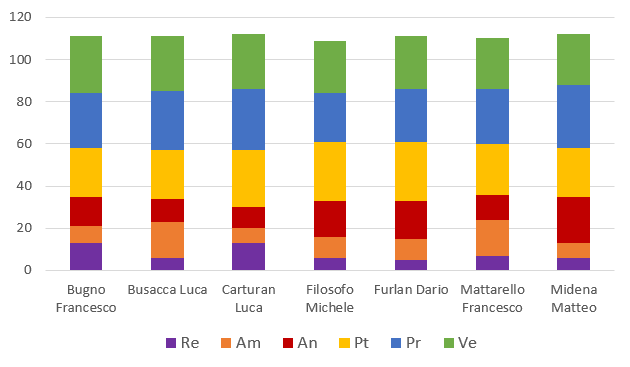
\includegraphics[scale=0.8]{immagini/ore_lavoro_preventivo_finire_PB.png}
  \caption{Istogramma della distribuzione oraria totale rendicontata - Preventivo a finire}
\end{figure}


\begin{table}[H]
  \centering
  \renewcommand{\arraystretch}{1.8}
  \rowcolors{2}{green!100!black!40}{green!100!black!30}
  \begin{tabular}{c|c|c}
    \rowcolor[HTML]{125E28}
    \multicolumn{1}{c}{\color[HTML]{FFFFFF}\textbf{Ruolo}}
                    & \multicolumn{1}{c}{\color[HTML]{FFFFFF}\textbf{Ore}}
                    & \multicolumn{1}{c}{\color[HTML]{FFFFFF}\textbf{Costo (€)}}                                \\
    \hline
    Responsabile    & 56 (+2)                                                    & 1680,00  (+60,00)            \\
    Amministratore  & 76 (+5)                                                    & 1520,00 (+100,00)            \\
    Analista        & 104 (+1)                                                   & 2600,00 (+25,00)             \\
    Progettista     & 176 (+25)                                                  & 4400,00 (+625,00)            \\
    Programmatore   & 187 (+33)                                                  & 2805,00 (+495,00)            \\
    Verificatore    & 177 (+11)                                                  & 2655,00 (+165,00)            \\
    \textbf{Totale} & \textbf{776 (+77)}                                         & \textbf{15660,00 (+1470,00)} \\
  \end{tabular}
  \caption{Prospetto delle ore e dei costi delle ore rendicontate - Preventivo a finire}
\end{table}

\begin{figure}[H]
  \centering
  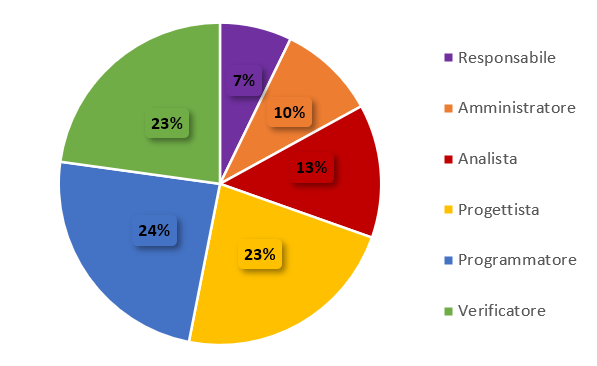
\includegraphics[scale=0.8]{immagini/ore_ruolo_preventivo_finire_PB.png}
  \caption{Areogramma delle ore per ruolo rendicontate sul totale - Preventivo a finire}
\end{figure}

Il carico di ore a persona è notevolmente aumentato ed il preventivo a finire sale a 15660,00€.


